%\documentclass[preprint,tightenlines,showpacs,showkeys,floatfix,
%nofootinbib,superscriptaddress,fleqn]{revtex4} 
\documentclass[tightenlines,floatfix,nofootinbib,superscriptaddress,fleqn]{revtex4}  
%\documentclass[aps,epsfig,tightlines,fleqn]{revtex4}
\usepackage{kotex}
\usepackage[HWP]{dhucs-interword}
\usepackage[dvips]{color}
\usepackage{graphicx}
\usepackage{bm}
%\usepackage{fancyhdr}
%\usepackage{dcolumn}
\usepackage{defcolor}
\usepackage{amsmath}
\usepackage{amsfonts}
\usepackage{amssymb}
\usepackage{amscd}
\usepackage{amsthm}
\usepackage[utf8]{inputenc}
%\pagestyle{fancy}

\begin{document}

\title{\Large 2022년 2학기 물리학 II}
\author{김현철\footnote{Office: 5S-436D (면담시간 매주
    수요일-16:15$\sim$19:00)}} 
\email{hchkim@inha.ac.kr}
\affiliation{Hadron Theory Group, Department of Physics,
  Inha  University, Incheon 22212, Republic of Korea }
\date{Autumn Semester, 2022}

\maketitle

\section*{\large Quiz 10}
\noindent {\bf 문제 1 [20pt]:} 
그림~\ref{fig:1}과 같이 간격이 $d=1.00$ m인 2개의 긴 직선 도선에
지면에서 나오는 방향으로 각각 전류 $I_1=0.600$ A와 $I_2=0.400$ A가
흐른다. 두 직선 도선 사이에 작용하는 단위길이당 힘의 크기와 방향을
구하여라. 이때 두 직선 도선 사이에 전류가 흐르는 제3의 도선을 두었을
때 이 도선이 받는 힘의 합력이 0이 되는 $x$축상의 위치는 어느 곳인가? 
\begin{figure}[htp]
  \centering
  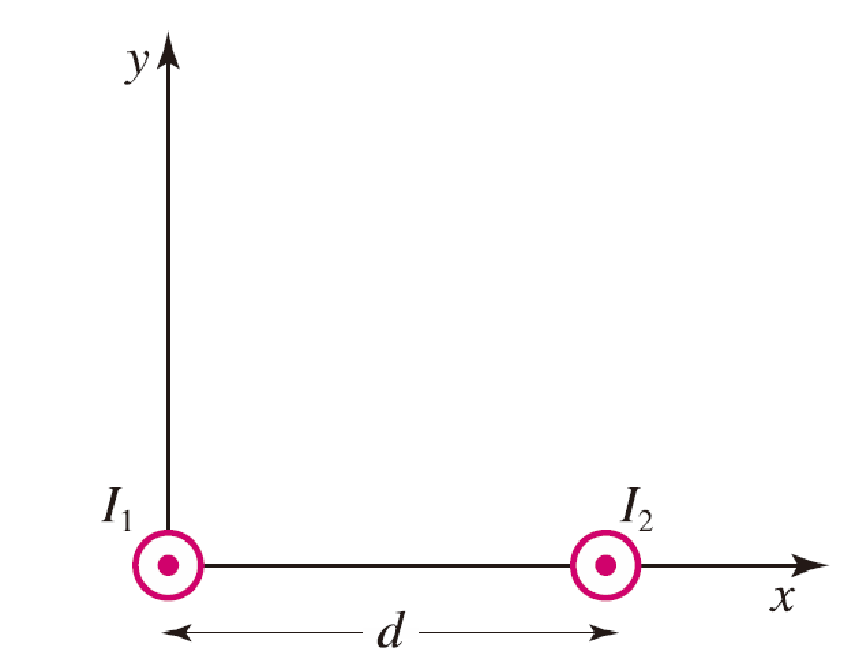
\includegraphics[scale=0.4]{qfig10-20221005-1.pdf}
  \caption{\textbf{문제 1}}
  \label{fig:1}
\end{figure}

\noindent {\bf 풀이 : } 
우선 두 직선 도선 사이에 작용하는 단위길이당 힘의 크기를 구하자. 도선의 길이를 $L$이라 하면
비오-사바르 법칙에 의해 두 도선이 서로에 의해 받는 힘 $\vec{F}_{12}$와 $\vec{F}_{21}$은
\begin{align}
  \vec{F}_{12} = I_1\vec{L}\times \vec{B_2},\,\,\,
  \vec{F}_{21} = I_2\vec{L}\times \vec{B_1}
\end{align}
이다.$\vec{F}_{12}$는 전류 $I_1$이 흐르는 도선이 받는 힘이고 $\vec{F}_{21}$는
전류 $I_2$가 흐르는 도선이 받는 힘이다.  전류의 방향이
$\hat{\bm k}$이므로 도선의 길이에 대한 벡터 $\vec{L}$은
\begin{align}
  \vec{L} = -L~\hat{\bm k}
\end{align}
이고 자기장 $\vec{B_1}$과 $\vec{B_2}$는 각각 직선 도선에 흐르는 전류 $I_1$, $I_2$에 
의해 생성되는 자기장이므로
\begin{align}
  \vec{B}_1 =  \frac{\mu_0 I_1}{2\pi d}\hat{\bm \phi},\,\,\,
  \vec{B}_2 =  \frac{\mu_0 I_2}{2\pi d}\hat{\bm \phi}
\end{align}
인데 각 도선의 위치에 작용하는 자기장의 방향을 고려하면 $\hat{\bm \phi}$는 
$\hat{\bm j}$에 평행하다. 따라서
\begin{align}
  \vec{B}_1 =  \frac{\mu_0 I_1}{2\pi d}~\hat{\bm j},\,\,\,
  \vec{B}_2 =  -\frac{\mu_0 I_2}{2\pi d}~\hat{\bm j}
\end{align} 
로 쓸 수 있다. 따라서 각 도선에 작용하는 힘 $\vec{F}_{12}$, $\vec{F}_{21}$은
\begin{align}
  \vec{F}_{12} = \frac{\mu_0I_1 I_2 L}{2\pi d}~\hat{\bm i}
  ,\,\,\,
  \vec{F}_{21} = -\frac{\mu_0I_1 I_2 L}{2\pi d}~\hat{\bm i}
\end{align}
이고 단위길이당 힘의 크기는
\begin{align}
  \begin{split}
    \frac{\vec{F}_{12}}{L} &= \frac{\mu_0I_1 I_2 }{2\pi d}~\hat{\bm i}
    ,\,\,\,
    \frac{\vec{F}_{21}}{L} = -\frac{\mu_0I_1 I_2 }{2\pi d}~\hat{\bm i} \\
    \frac{\mu_0I_1 I_2 }{2\pi d} &= \frac{(4\pi\times 10^{-7}~\mathrm{T\cdot m/A})
    (0.600~\mathrm{A}) (0.400~\mathrm{A}) }{2\pi (1.00~\mathrm{m})}
    =4.8\times 10^{-8}~\mathrm{N}
  \end{split}
\end{align}
$4.8\times 10^{-8}~\mathrm{N}$이며 방향은 각 도선을 끌어당기는 방향이다. 이제 제 3의 도선을 
두었을 때 힘의 합력이 $0$인 $x$축 상의 위치를 구해보자. 전류는 지면에서 나오는 방향으로 흐른다고
가정한다. $x$축 위 두 도선 사이인 $x=x_0$에 위치한 제 3의 도선에 전류 $I_3$이 흐르고 있을 때 
전류 $I_1$이 흐르는 도선에 의한 힘 $\vec{F}_1$과 전류 $I_2$가 흐르는 도선에 의한 힘 
$\vec{F}_2$는
\begin{align}
  \vec{F}_1 = \frac{\mu_0I_1 I_3 L}{2\pi x_0}~\hat{\bm i},\,\,\,
  \vec{F}_2 =-\frac{\mu_0I_2 I_3 L}{2\pi (d-x_0)}~\hat{\bm i}
\end{align}
이고 도선이 받는 힘의 합력이 0이 되어야 하므로
\begin{align}
  \vec{F}_1+\vec{F}_2=\vec{0} \Longrightarrow
  \frac{\mu_0I_1 I_3 L}{2\pi x_0}=\frac{\mu_0I_2 I_3 L}{2\pi (d-x_0)}
\end{align}
를 만족하는 $x_0$를 찾아야 한다. 식을 정리하면
\begin{align}
  \frac{I_1}{x_0}=\frac{I_2}{d-x_0}\Longrightarrow
  x_0 = \frac{I_1d}{I_1+I_2} = \frac{(0.600~\mathrm{A})(1.00~\mathrm{m})}
  {(0.600~\mathrm{A}+0.400~\mathrm{A})}=0.600~\mathrm{m}
\end{align}
를 얻는다. 따라서 도선이 받는 힘의 합력이 0이 되는 위치는 $0.600~\mathrm{m}$이다.
\vspace{1cm}

\noindent {\bf 문제 2 [30pt]:}
구름과 땅 사이에 수직으로 벼락이 칠 때 순간적으로 $1.00\times 10^4$
A의 전류가 흐른다고 한다. 벼락으로부터 100.0 m 떨어진 산 위에서 벼락에
의해 순간적으로 형성되는 자기장의 크기를 계산하라.

\noindent {\bf 풀이 : } 

\vspace{1cm}

\noindent {\bf 문제 3 [50pt]:}
반지름이 6.00 cm인 원형 회로의 면에 수직으로 통과하는 균일한 자기장이
0.0100 s 동안에 5.30 T에서 0 T까지 일정한 비율로 변하였다. 그동안
회로에 유도되는 기전력을 구하여라.

\noindent {\bf 풀이 : } 
\vspace{1cm}

\noindent {\bf 문제 4 [50pt]:}
각 변의 길이가 $2.00$ m인 정사각형 고리 전류가
그림~\ref{fig:2}에서처럼 대각선으로 절반만 자기장에 수직한 면에 
놓여있다. 이 고리에는 기전력이 $\mathcal{E}_{\mathrm{emf}}$인 이상적인
배터리가 연결되어 있다. 자기장은 시간에 대해 $B=0.02420-0.820t$와 같이
변한다. 여기서 $B$의 단위는 테슬라이고, 시간은 초로 주어진다. 
\begin{figure}[htp]
  \centering
  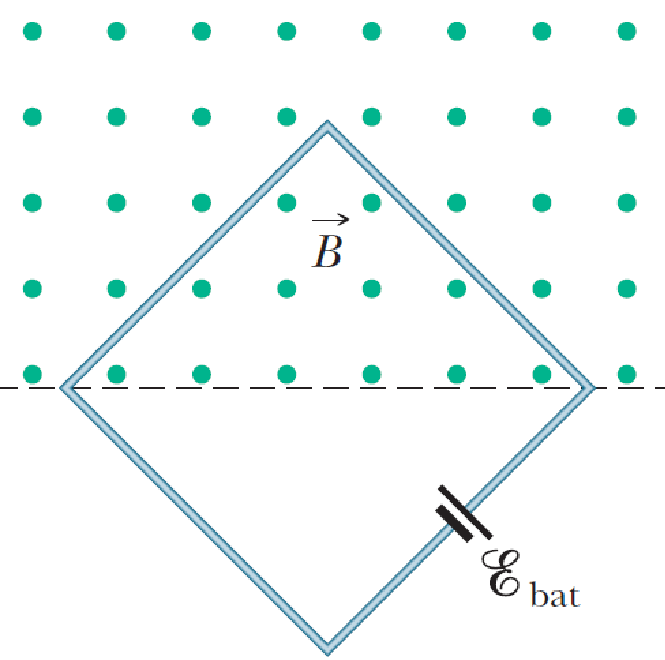
\includegraphics[scale=0.4]{qfig10-20221005-2.pdf}
  \caption{\textbf{문제 4}}
  \label{fig:2}
\end{figure}
\begin{itemize}
\item[(가)] 이 도선에 가해지는 알짜 기전력은 얼마인가?  
\item[(나)] 이 고리를 흐르는 전류는 어떤 방향으로 흐르는가? 
\end{itemize}
\vspace{1cm}
\noindent {\bf 풀이 : } 
\begin{itemize}
  \item[(가)] 도선 내 자기장이 시간에 따라 줄어들기 때문에 렌츠의 법칙에 의해 도선에는
  자기장이 증가하도록 하는 방향인 반시계 방향으로 기전력이 생성된다. 도선 고리 안을 통과하는
  자기장의 선속을 $\Phi_B$라고 하면 기전력의 크기 
  $\mathcal{E}$는
  \begin{align}
    \mathcal{E} = -\frac{d\Phi_B}{dt} = -A\frac{dB}{dt}
  \end{align}
  이다. 여기서 $A$는 자기장이 통과하는 면적이고 $B$는 자기장의 크기이다. $\mathcal{E}$를
  구해보면
  \begin{align}
    \mathcal{E} = (-2.00~\mathrm{m^2})\frac{d(0.02420-0.820t~\mathrm{T})}{dt}
    =1.64~\mathrm{T\cdot m^2/s}=1.64~\mathrm{V}
  \end{align}
  이고 이상적인 배터리의 기전력 $\mathcal{E}_{\mathrm{emf}}$ 또한 시계 반대 방향의 기전력을
  생성하므로 알짜 기전력 $\mathcal{E}_{tot}$는
  \begin{align}
    \mathcal{E}_{tot} = \mathcal{E}+\mathcal{E}_{\mathrm{emf}}
    =1.64~\mathrm{V} + \mathcal{E}_{\mathrm{emf}}
  \end{align}
  이다.
  \item[(나)] 기전력이 시계 반대 방향으로 발생하므로 전류 또한 기전력을 따라 시계 반대 방향으로
  흐른다.
\end{itemize}
\end{document}

